\documentclass{article}
\usepackage[utf8]{inputenc}
\usepackage{amsmath,amsthm,amsfonts}
\usepackage{graphicx}

\newtheorem{theorem}{Theorem}[section]
\newtheorem{corollary}{Corollary}[theorem]

\newcommand{\R}{\mathbb{R}}
\newcommand{\cv}[2]{
    \begin{bmatrix}
        #1\\
        #2\\
    \end{bmatrix}
}

\begin{document}
\begin{enumerate}
\item $e^{\pi i}$
\item $$
e = \lim_{n \to \infty}\left(1 + \frac{1}{n}\right)^n = \lim_{n \to \infty} \frac{\sqrt{n}}{n!}
$$

\item $$
e = \sum_{n=0}^{\infty} \frac{1}{n!}
$$

\begin{align}
\label{e-definiton}
    e &= 2 + \frac{1}{\frac{1}{2 + \ddots}} \\
    &= \lim_{n \to 0} (1 + t)^ \frac{1}{n}
\end{align}

\begin{equation}
\begin{split}
    e &= 2 + \frac{1}{\frac{1}{2 + \ddots}} \\
    &= \lim_{n \to 0} (1 + t)^ \frac{1}{n}
\end{split}
\end{equation}

\end{enumerate}

$$\int_{a}^{b} f(x)dx$$

$$\iiint f(x, y, z)dxdydz$$

$$\vec{v} = <v_1, v_2>$$

$$\vec{v} \cdot \vec{w}$$

$$
\begin{bmatrix}
    1 & 2 \\
    3 & 4 \\
    4 & 5
\end{bmatrix}
$$

\newpage
\begin{table}
\caption{Le table}    
\begin{center}
\begin{tabular}{|c|r|}
    \hline
    1 & 2 \\\hline
    4 & 5 \\\hline
\end{tabular}
\end{center}
\end{table}

def: \ref{e-definiton}

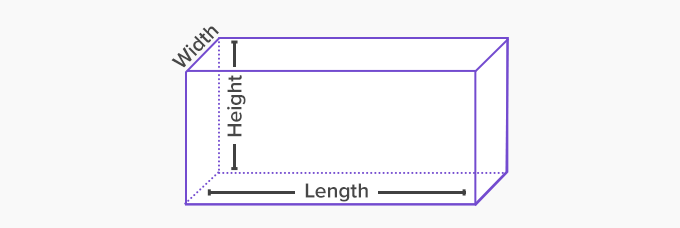
\includegraphics[scale=0.5]{length.png}

\begin{figure}
    \centering
    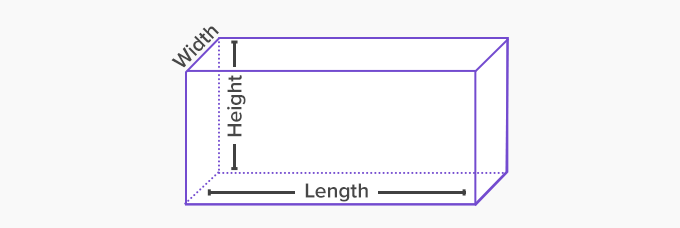
\includegraphics[width=0.8\textwidth]{length.png}
    \caption{YES}
    \label{YES}
\end{figure}

So proud of \ref{YES}

\section{Theorems}
\begin{theorem}{YES Theorem}
YES 
\end{theorem}
\begin{proof}
   hmmmm 
\end{proof}

\begin{corollary}
   hmm 
\end{corollary}

\begin{theorem}
YEAH
\end{theorem}

Real numbers $\R$
\cv{1}{2}
\end{document}
